\documentclass[11pt]{article}            % Report class in 11 points
\parindent0pt  \parskip10pt             % make block paragraphs
\usepackage{graphicx}
\usepackage{listings}
\graphicspath{ {images/} }
\usepackage{graphicx} %  graphics header file
\begin{document}
\begin{titlepage}
    \centering
  \vfill
    
\includegraphics[width=8cm]{uni_logo.png} \\ 
	\vskip2cm
    {\bfseries\Large
	Artificial Intelligence \\ (CS13217)\\
	
	\vskip2cm
	Lab Report 4
	 
	\vskip2cm
	}    

\begin{center}
\begin{tabular}{ l l  } 

Name: Kanza Afzal \\ 
Registration \#: & CSU-XS18-132 \\ 
Lab Report \#: & 04 \\ 
 Dated:&16-04-2018\\ 
Submitted To:& Mr. Usman Ahmed\\ 

 %\hline
\end{tabular}
\end{center}
    \v
    The University of Lahore, Islamabad Campus\\
Department of Computer Science \& Information Technology
\end{titlepage}


    
    {\bfseries\Large
\centering
	Experiment \# 4 \\

Implementing Breadth First  Search Problem\\
	
	}    
 \vskip1cm
 \textbf {Objective}\\  To understand and implement the Breadth First Search
 
 \textbf {Software Tool} \\
1.  \\pythaon

\section{Theory }              

\section{Task}  
\subsection{Procedure: Task 1 }     

\begin{figure*}Breadth-first search (BFS) is an algorithm for traversing or searching tree or graph data structures. It starts at the tree root (or some arbitrary node of a graph, sometimes referred to as a 'search key'[1]) and explores the neighbor nodes first, before moving to the next level neighbours.
\centering
  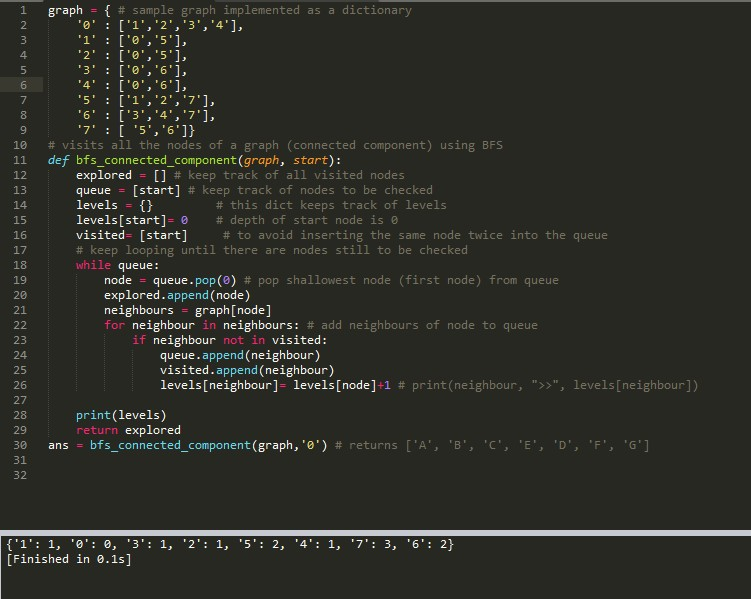
\includegraphics[width=35cm,height=16cm,keepaspectratio]{3.jpg}
\caption{Iplementation of Breadth First Search}
\label{Figure:3}    
\end{figure*}
To traverse all the nodes in the graph using BFS technique.

\subsection{Procedure: Task 2 }     

\begin{lstlisting}[language=Python]
graph = { # sample graph implemented as a dictionary
    '0' : ['1','2','3','4'],
    '1' : ['0','5'],
    '2' : ['0','5'],
    '3' : ['0','6'],
    '4' : ['0','6'],
    '5' : ['1','2','7'],
    '6' : ['3','4','7'],
    '7' : [ '5','6']}
# visits all the nodes of a graph (connected component) using BFS
def bfs_connected_component(graph, start):
    explored = [] # keep track of all visited nodes
    queue = [start] # keep track of nodes to be checked
    levels = {}         # this dict keeps track of levels
    levels[start]= 0    # depth of start node is 0
    visited= [start]     # to avoid inserting the same node twice into the queue
    # keep looping until there are nodes still to be checked
    while queue:
        node = queue.pop(0) # pop shallowest node (first node) from queue
        explored.append(node)
        neighbours = graph[node]
        for neighbour in neighbours: # add neighbours of node to queue
            if neighbour not in visited:
                queue.append(neighbour)
                visited.append(neighbour)
                levels[neighbour]= levels[node]+1 # print(neighbour, ">>", levels[neighbour])
                
    print(levels)
    return explored
ans = bfs_connected_component(graph,'0') # returns ['A', 'B', 'C', 'E', 'D', 'F', 'G']

\end{lstlisting}

\section{Conclusion}  
Breadth first search will never get trapped exploring the useless path forever.
If there is a solution, BFS will definitely find it out.
If there is more than one solution then BFS can find the minimal one that requires less number of steps.
   

 
\end{document}                          % The required last line
